\documentclass{article}

\usepackage{amsmath, amsthm, amssymb, amsfonts}
\usepackage{thmtools}
\usepackage{graphicx}
\usepackage{caption, subcaption}
\usepackage{setspace}
\usepackage{geometry}
\usepackage{float}
\usepackage[colorlinks=true, linkcolor=blue]{hyperref}
\usepackage[utf8]{inputenc}
\usepackage[english]{babel}
\usepackage{framed}
\usepackage[dvipsnames]{xcolor}
\usepackage{tcolorbox}
\usepackage{subcaption}
\usepackage{amssymb}
\usepackage{cite}
\usepackage{booktabs}
\usepackage{multirow}
\usepackage{anyfontsize}
\usepackage{tabularx}
\usepackage{adjustbox}
\usepackage{abstract}
\usepackage{array}

\colorlet{LightGray}{White!90!Periwinkle}
\colorlet{LightOrange}{Orange!15}
\colorlet{LightGreen}{Green!15}

\newcommand{\HRule}[1]{\rule{\linewidth}{#1}}

\declaretheoremstyle[name=Theorem,]{thmsty}
\declaretheorem[style=thmsty,numberwithin=section]{theorem}
\tcolorboxenvironment{theorem}{colback=LightGray}

\declaretheoremstyle[name=Proposition,]{prosty}
\declaretheorem[style=prosty,numberlike=theorem]{proposition}
\tcolorboxenvironment{proposition}{colback=LightOrange}

\declaretheoremstyle[name=Principle,]{prcpsty}
\declaretheorem[style=prcpsty,numberlike=theorem]{principle}
\tcolorboxenvironment{principle}{colback=LightGreen}

\setstretch{1.2}
\geometry{
    textheight=9in,
    textwidth=5.5in,
    top=1in,
    headheight=12pt,
    headsep=25pt,
    footskip=30pt
}

% ------------------------------------------------------------------------------

\begin{document}

    % Cover Page and ToC
    \title{ \normalsize \textsc{}
\\ [2.0cm]
\HRule{1.5pt} \\
\LARGE \textbf{\uppercase{Machine Learning and Pattern Recognition Report}
\HRule{2.0pt} \\ [0.6cm] \LARGE{Fingerprint Spoofing Detection} \vspace*{10\baselineskip}}
}
\date{}
\author{\textbf{Antonio Iorio} \\
Who? \\
Where? \\
When?}

\maketitle
\newpage

\tableofcontents
\newpage

    %Introduction

    \paragraph{Introduction}
    The project task consists of a binary classification problem.
    The goal is to perform fingerprint spoofing detection, i.e.\ to identify genuine vs counterfeit fingerprint images.
    The dataset consists of labeled samples corresponding to the genuine (True, label 1) class and the fake (False, label 0) class.
    The samples are computed by a feature extractor that summarizes high-level characteristics of a fingerprint
    image.
    The data is 6-dimensional.

%    Dataset Analysis


    \section{Dataset Analysis}
    \label{sec:datasetAnalysis}
    %! Author = antonio
%! Date = 7/1/24

In our analysis process, one first begins to represent what are the data related to the various features
and how among the various features the data are distributed by making a visual representation in pairs of features.

\begin{enumerate}
%    FEATURE 1 AND 2
    \item Starting with the analysis of the first two features and creating a histogram and a scatter
    \autoref{fig:feature1vs2}, one can see:
    \begin{itemize}
        \item Both features overlap
        \item Follow a Gaussian distribution
        \item Feature 1 has a peak at [-0.213, 0.276] and it is worth 0.541 for the false class, instead for Feature 2
        the peak at [-0.402, 0.165] and it is worth 0.516 for the true class.
    \end{itemize}
    Seeing \autoref{fig:feature1vs2} again, it would appear that \autoref{fig:feature1vs2a} and
    \autoref{fig:feature1vs2b} appear to be visually the same but in b they are represented centred
    which as can be seen is quite similar because Feature 1 has \(\mu = 0.00170711\)
    and \(\sigma^2 = 1.00134304\), instead Feature 2 has \(\mu = 0.00503903\) and \(\sigma^2 =  0.9983527\)
    \begin{figure}[h!]
        \centering
        \begin{subfigure}[b]{0.4\linewidth}
            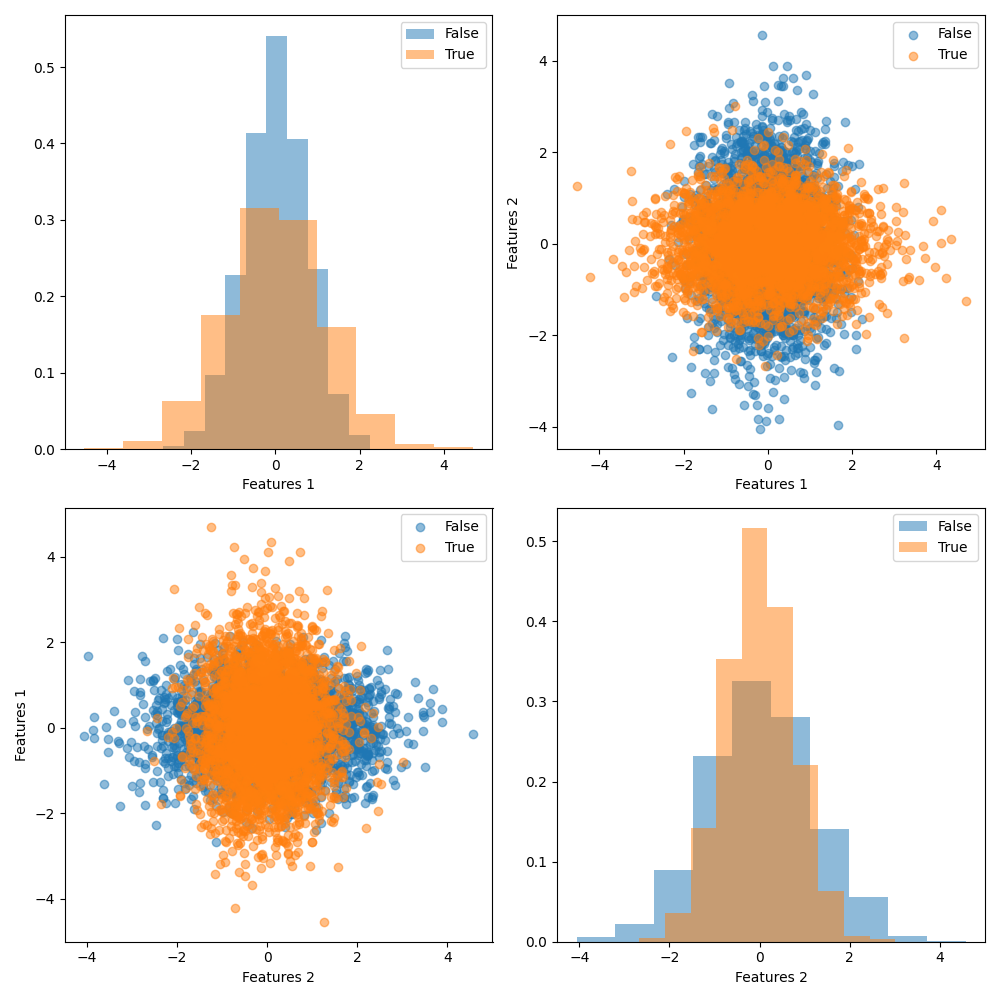
\includegraphics[width=\linewidth]{Lab/02. Lab 02/Images/01. Graphics Features 1_2 Without Mean}
            \caption{Without mean}
            \label{fig:feature1vs2a}
        \end{subfigure}
        \begin{subfigure}[b]{0.4\linewidth}
            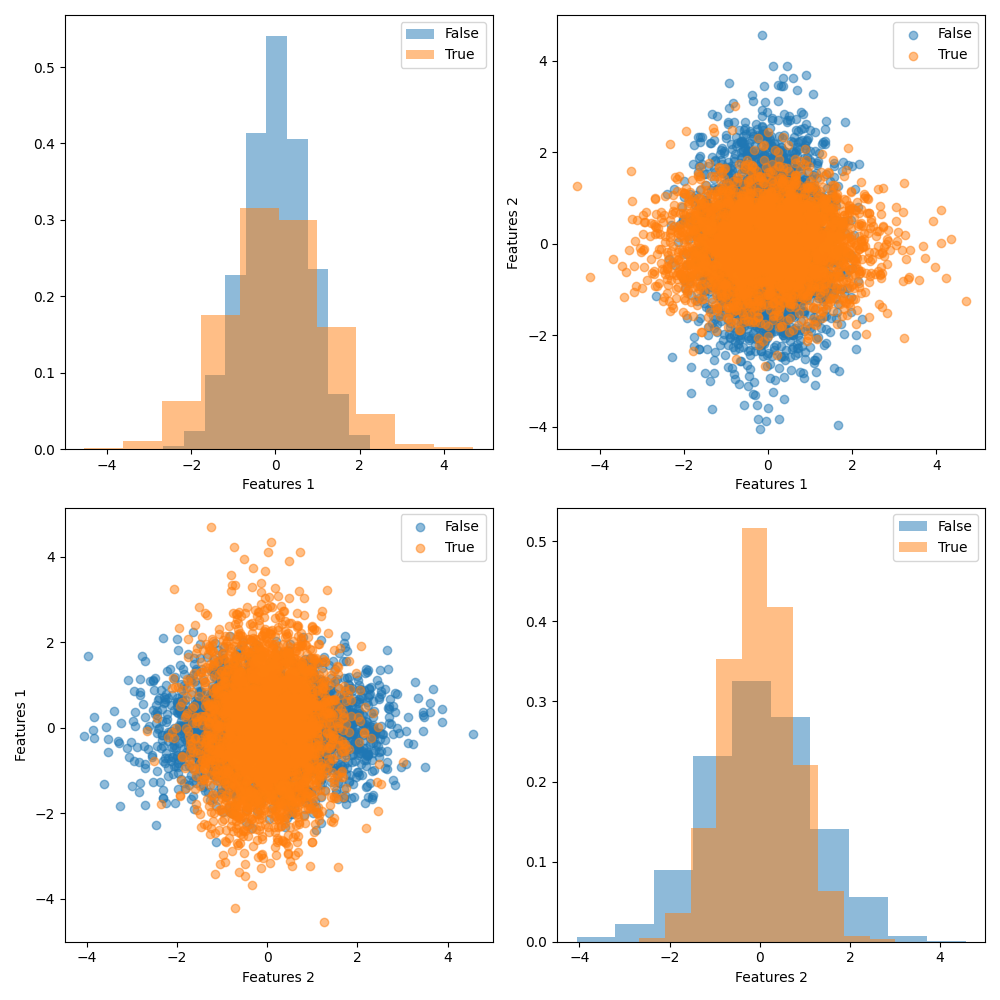
\includegraphics[width=\linewidth]{Lab/02. Lab 02/Images/02. Graphics Features 1_2 With Mean}
            \caption{With mean}
            \label{fig:feature1vs2b}
        \end{subfigure}
        \caption{Feature 1 vs Feature 2 - Without centering the data relative to the average (a)
            and with centering the data relative to the average (b)}
        \label{fig:feature1vs2}
    \end{figure}


%    FEATURE 3 AND 4
    \item For features 3 and 4, observed in \autoref{fig:feature3vs4}, on the other hand, they have:
    \begin{itemize}
        \item do not overlap like the previous two
        \item Follow a Gaussian distribution but the true and false labels are centred at different
        points
        \item Feature 3 has a peak at [-1.063, -0.568] and it is worth 0.517 for the false class,
        instead for Feature 4 the peak at [0.290, 0.783] and it is worth 0.525 for the false class.
    \end{itemize}
    Seeing \autoref{fig:feature3vs4a} and \autoref{fig:feature3vs4b}, data are already similar because, the mean
    calculated with reference to the two classes is close to 0, in fact:
    Feature 3 has \(\mu = -0.00560753\) and \(\sigma^2 = 1.0024818\), instead
    Feature 4 has \(\mu = 0.00109537\) and \(\sigma^2 = 0.99029389\)
    \begin{figure}[h!]
        \centering
        \begin{subfigure}[b]{0.4\linewidth}
            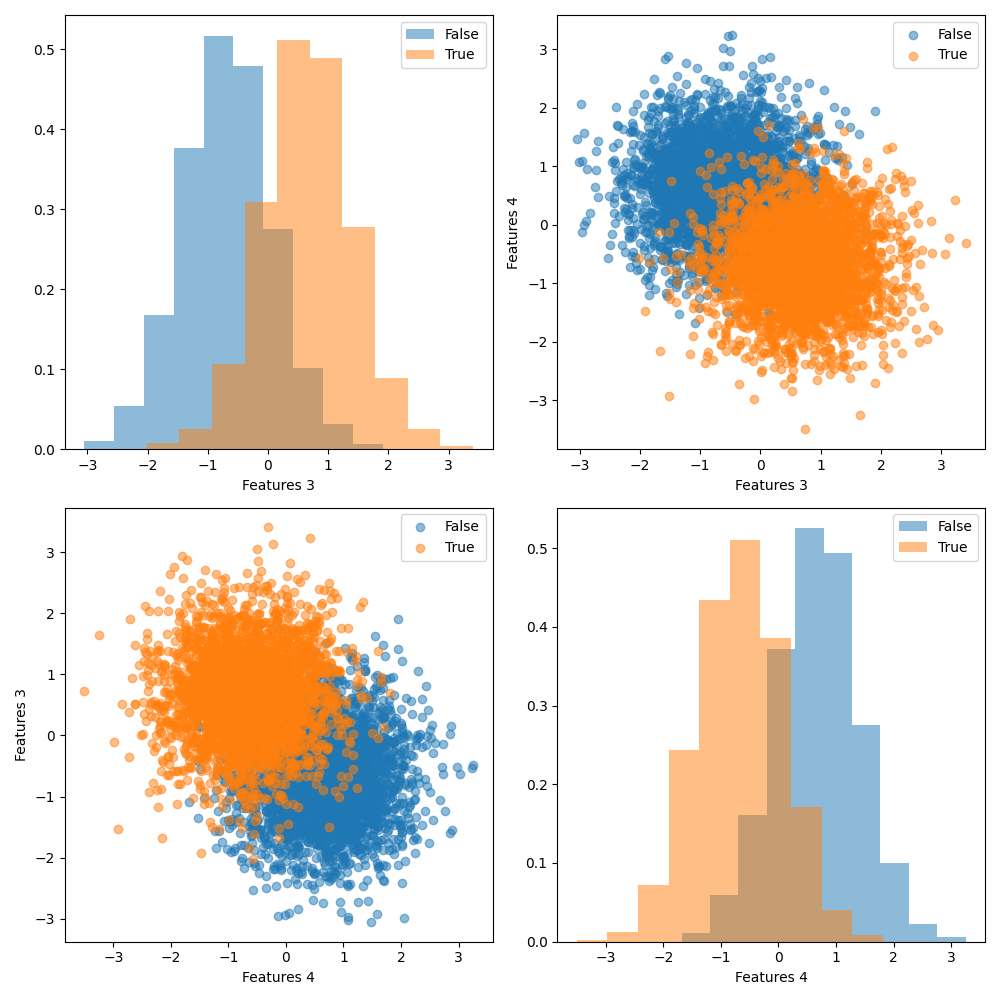
\includegraphics[width=\linewidth]{Lab/02. Lab 02/Images/03. Graphics Features 3_4 Without Mean}
            \caption{Without mean}
            \label{fig:feature3vs4a}
        \end{subfigure}
        \begin{subfigure}[b]{0.4\linewidth}
            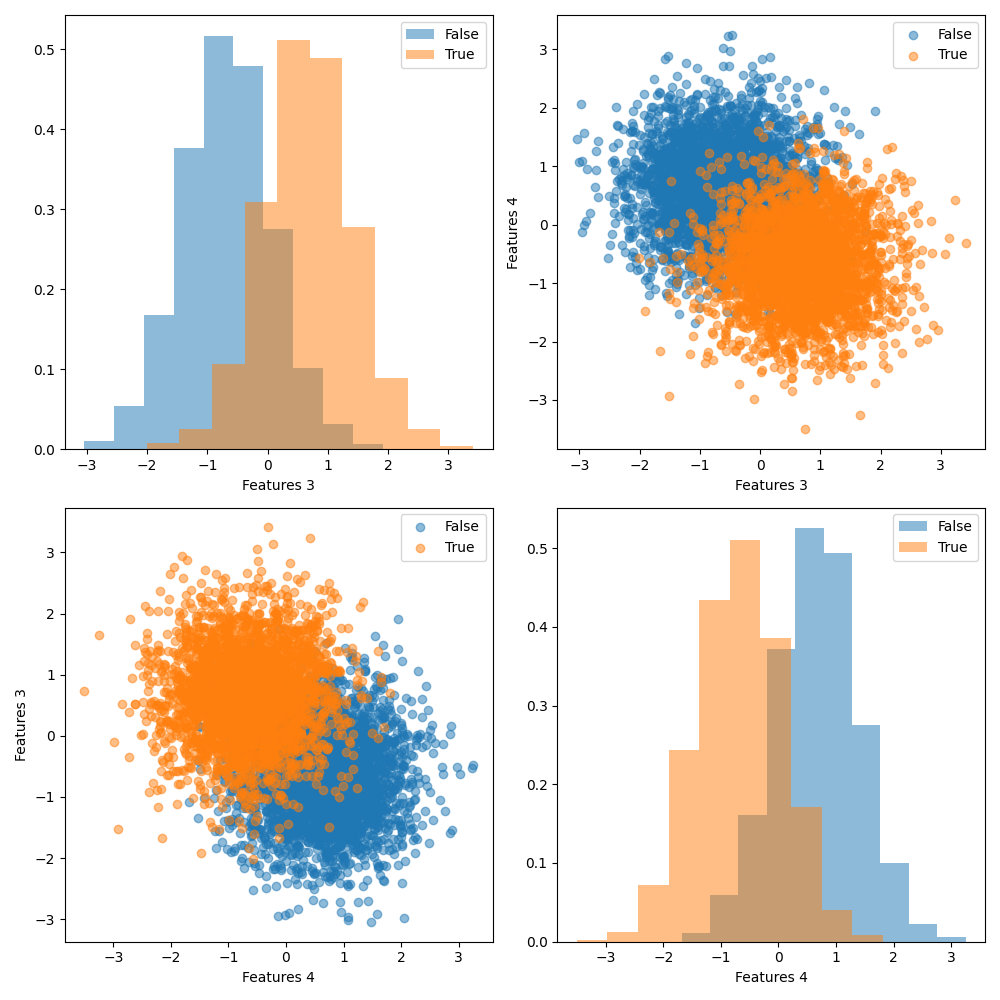
\includegraphics[width=\linewidth]{Lab/02. Lab 02/Images/04. Graphics Features 3_4 With Mean}
            \caption{With mean}
            \label{fig:feature3vs4b}
        \end{subfigure}
        \caption{Feature 3 vs Feature 4 - Without centering the data relative to the average (a)
            and with centering the data relative to the average (b)}
        \label{fig:feature3vs4}
    \end{figure}


%    FEATURE 5 AND 6
    \item  For features 5 and 6, observed in \autoref{fig:feature5vs6}, one can see:
    \begin{itemize}
        \item Do not totally overlap
        \item For both features, the true labels don't follow a Gaussian distribution as opposed to the false ones,
        which could be more approximate
        \item Feature 5 has a peak at [-1.211, -0.783] and it is worth 0.572 for the true class, instead
        for Feature 6 has a peak at [-1.273, -0.817] and it is worth 0.553 for the true class.
    \end{itemize}
    Also in this other case, \autoref{fig:feature5vs6a} and \autoref{fig:feature5vs6b} are similar because again the
    average is close to 0.
    Feature 5 has \(\mu = -0.00700025\) and Feature 6 has \(\mu = 0.00910515\)

    \begin{figure}[t]
        \centering
        \begin{subfigure}[b]{0.4\linewidth}
            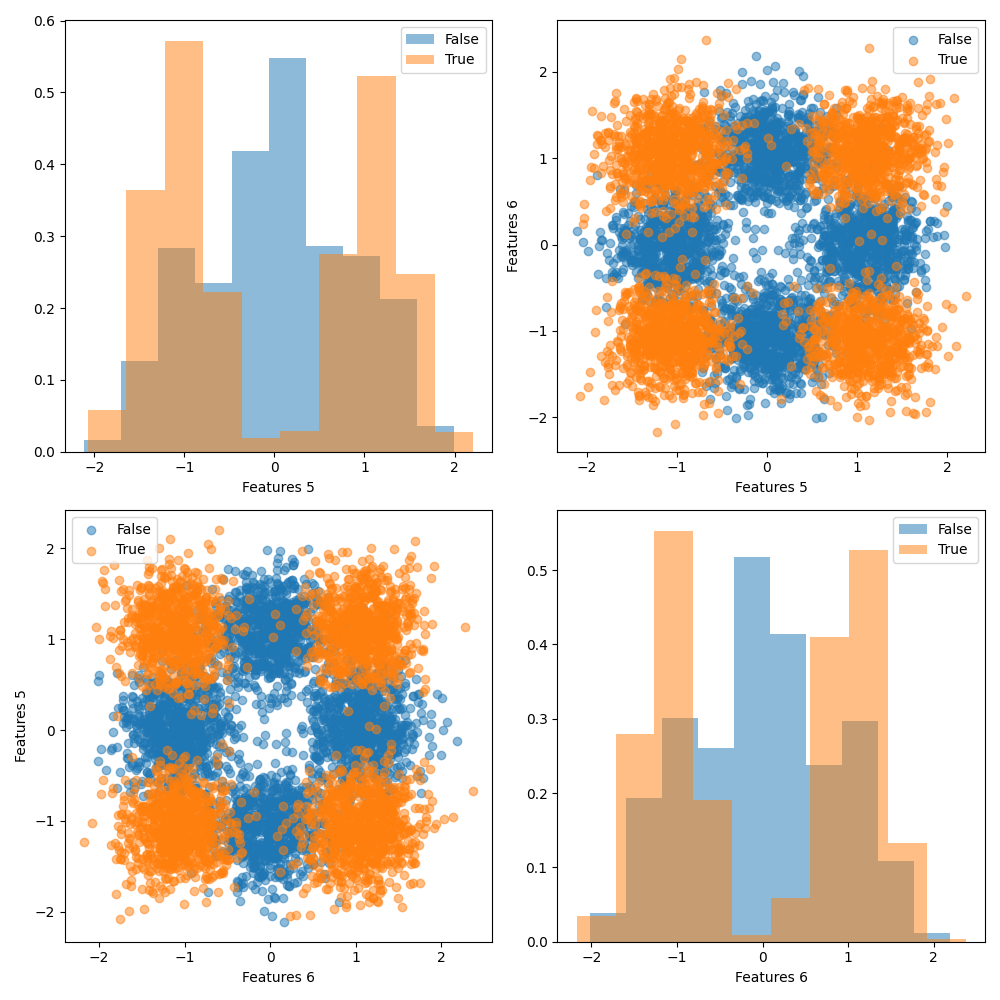
\includegraphics[width=\linewidth]{Lab/02. Lab 02/Images/05. Graphics Features 5_6 Without Mean}
            \caption{Without mean}
            \label{fig:feature5vs6a}
        \end{subfigure}
        \begin{subfigure}[b]{0.4\linewidth}
            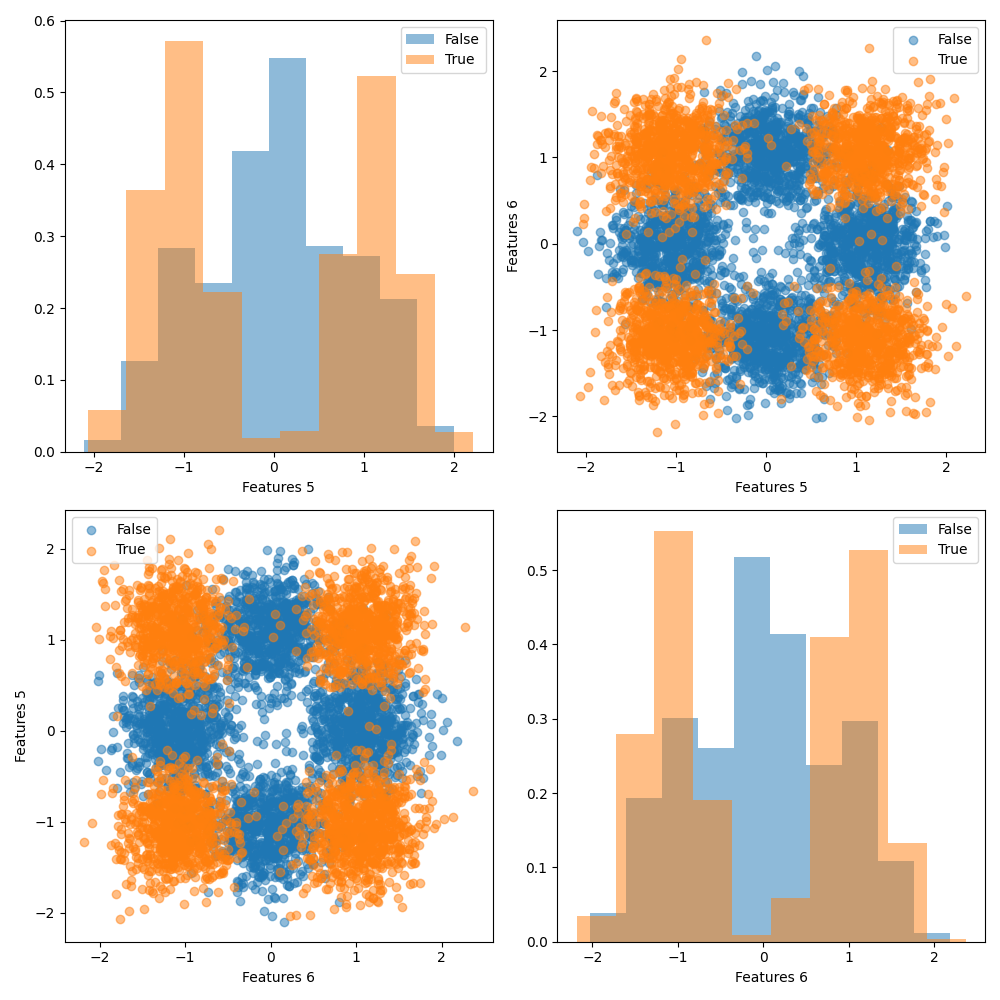
\includegraphics[width=\linewidth]{Lab/02. Lab 02/Images/06. Graphics Features 5_6 With Mean}
            \caption{With mean}
            \label{fig:feature5vs6b}
        \end{subfigure}
        \caption{Feature 5 vs Feature 6 - Without centering the data relative to the average (a)
            and with centering the data relative to the average (b)}
        \label{fig:feature5vs6}
    \end{figure}

\end{enumerate}


%    Dimensionality Reduction


    \section{Dimensionality Reduction}
    \label{sec:dimensionalityReduction}
    %! Author = antonio
%! Date = 7/2/24

Before proceeding with classification, two techniques of dimensionality reduction PCA and LDA can be analysed.
The goal is to find a subspace of the feature space that preserves most of the useful information, that is, mapping from
the \(n\text{–}dimensional\) feature space to \(m\text{–}dimensional\) space, with
\(m \ll n\)

% PCA

\subsection{PCA}
\label{subsec:pca} is an unsupervised technique.
Where starting from a dataset \(X = \{x_1, \dots,x_k\}\) and calculated average.
It starts with the empirical covariance matrix:
\begin{equation}
    C = \frac{1}{K} \sum (x_i - \bar{x})(x_i - \bar{x})^T
    \label{eq:covarianceMatrix}
\end{equation}

We compute the eigen-decomposition of \(C = U \Sigma U^T\) and project the data in the subspace
spanned by the \(m\) columns of \(U\) corresponding to the \(m\) largest eigenvalues.
\begin{equation}
    y_i = P^T(x_i - \bar{x})
    \label{eq:projection}
\end{equation}

where P is the matrix of the \(m\) columns of U associated to the m highest eigenvalues of \(C\).
A cross-validation approach can be used to figure out the optimal value of m to be selected.
To evaluate each eigenvalue, one would have to calculate the variance corresponding to the axis.
The percentage can be calculated as the rate between the sum of the m eigenvalues and the sum of all of them.
In \autoref{fig:percentageVariance} we can see how it changes in the project.
A good m, corresponds to that value which allows a percentage greater than 95\%, so in our case we would need all 6
features.

\begin{figure}[h!]
    \centering
    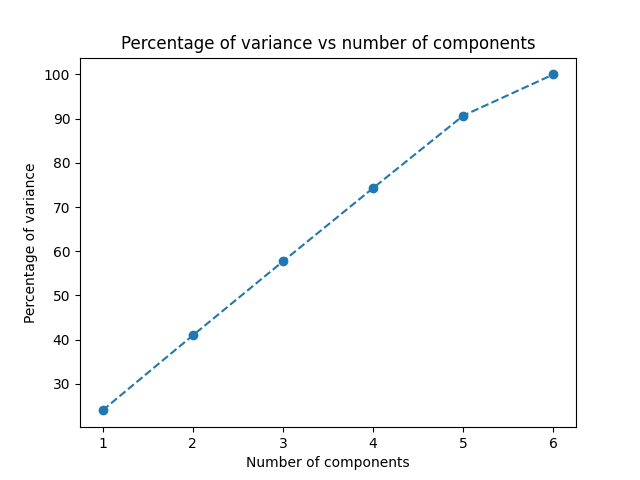
\includegraphics[width=0.5\linewidth]{Lab/03. Lab 03/Images/01. PercentageVariance_NumberOfComponents}
    \caption{Cross validation for PCA impact evaluation}
    \label{fig:percentageVariance}
\end{figure}

% LDA

\subsection{LDA}
\label{subsec:LDA} is a supervised technique.
To find a direction that has the best separation between classes, we measure spread between classes in terms of class covariance.
The objective is to maximize the \(between-class\) variability over \(within-class\) variability ratio for the transformed samples:
\begin{equation}
    \underset{w}{\max} \frac{w^T S_B w}{w^T S_W w}
    \label{eq:ldaFunct}
\end{equation}

where:
\begin{equation}
    S_B  \triangleq \frac{1}{N}\sum_{c=1}^{K} n_c (\mu_c - \mu)(\mu_c - \mu)^T
    \label{eq:betweenClass}
\end{equation}

\begin{equation}
    S_W \triangleq \frac{1}{N}\sum_{c=1}^{K} \sum_{i=1}^{n_c} (x_{c,i} - \mu_c)(x_{c,i} - \mu_c)^T
    \label{eq:withinClass}
\end{equation}

\(\mu\) is dataset mean, \(\mu_{c}\) is class mean, \(n_c\) is the number of samples in class \(c\), and \(N\) is the total number of samples.\\
The directions of LDA can be calculated by solving the generalised eigenvalue problem, as one wants to find the associated eigenvectors \(S_w^{-1}S_b\).
This method allows us to find at most C-1 discriminant directions, where C is the number of classes, since the objective of
LDA is to maximize the separation between classes.
In our case there are 2 classes so there is only one direction

% OUR PROJECT

\subsection{Our project}
\label{subsec:ourProject}
PCA and LDA are applied to the dataset, in particular, m = 6 is used, and in \autoref{fig:pcaLda} we can observe
what are the outcomes for the indicated directions.

\begin{figure}[h]
    \centering
    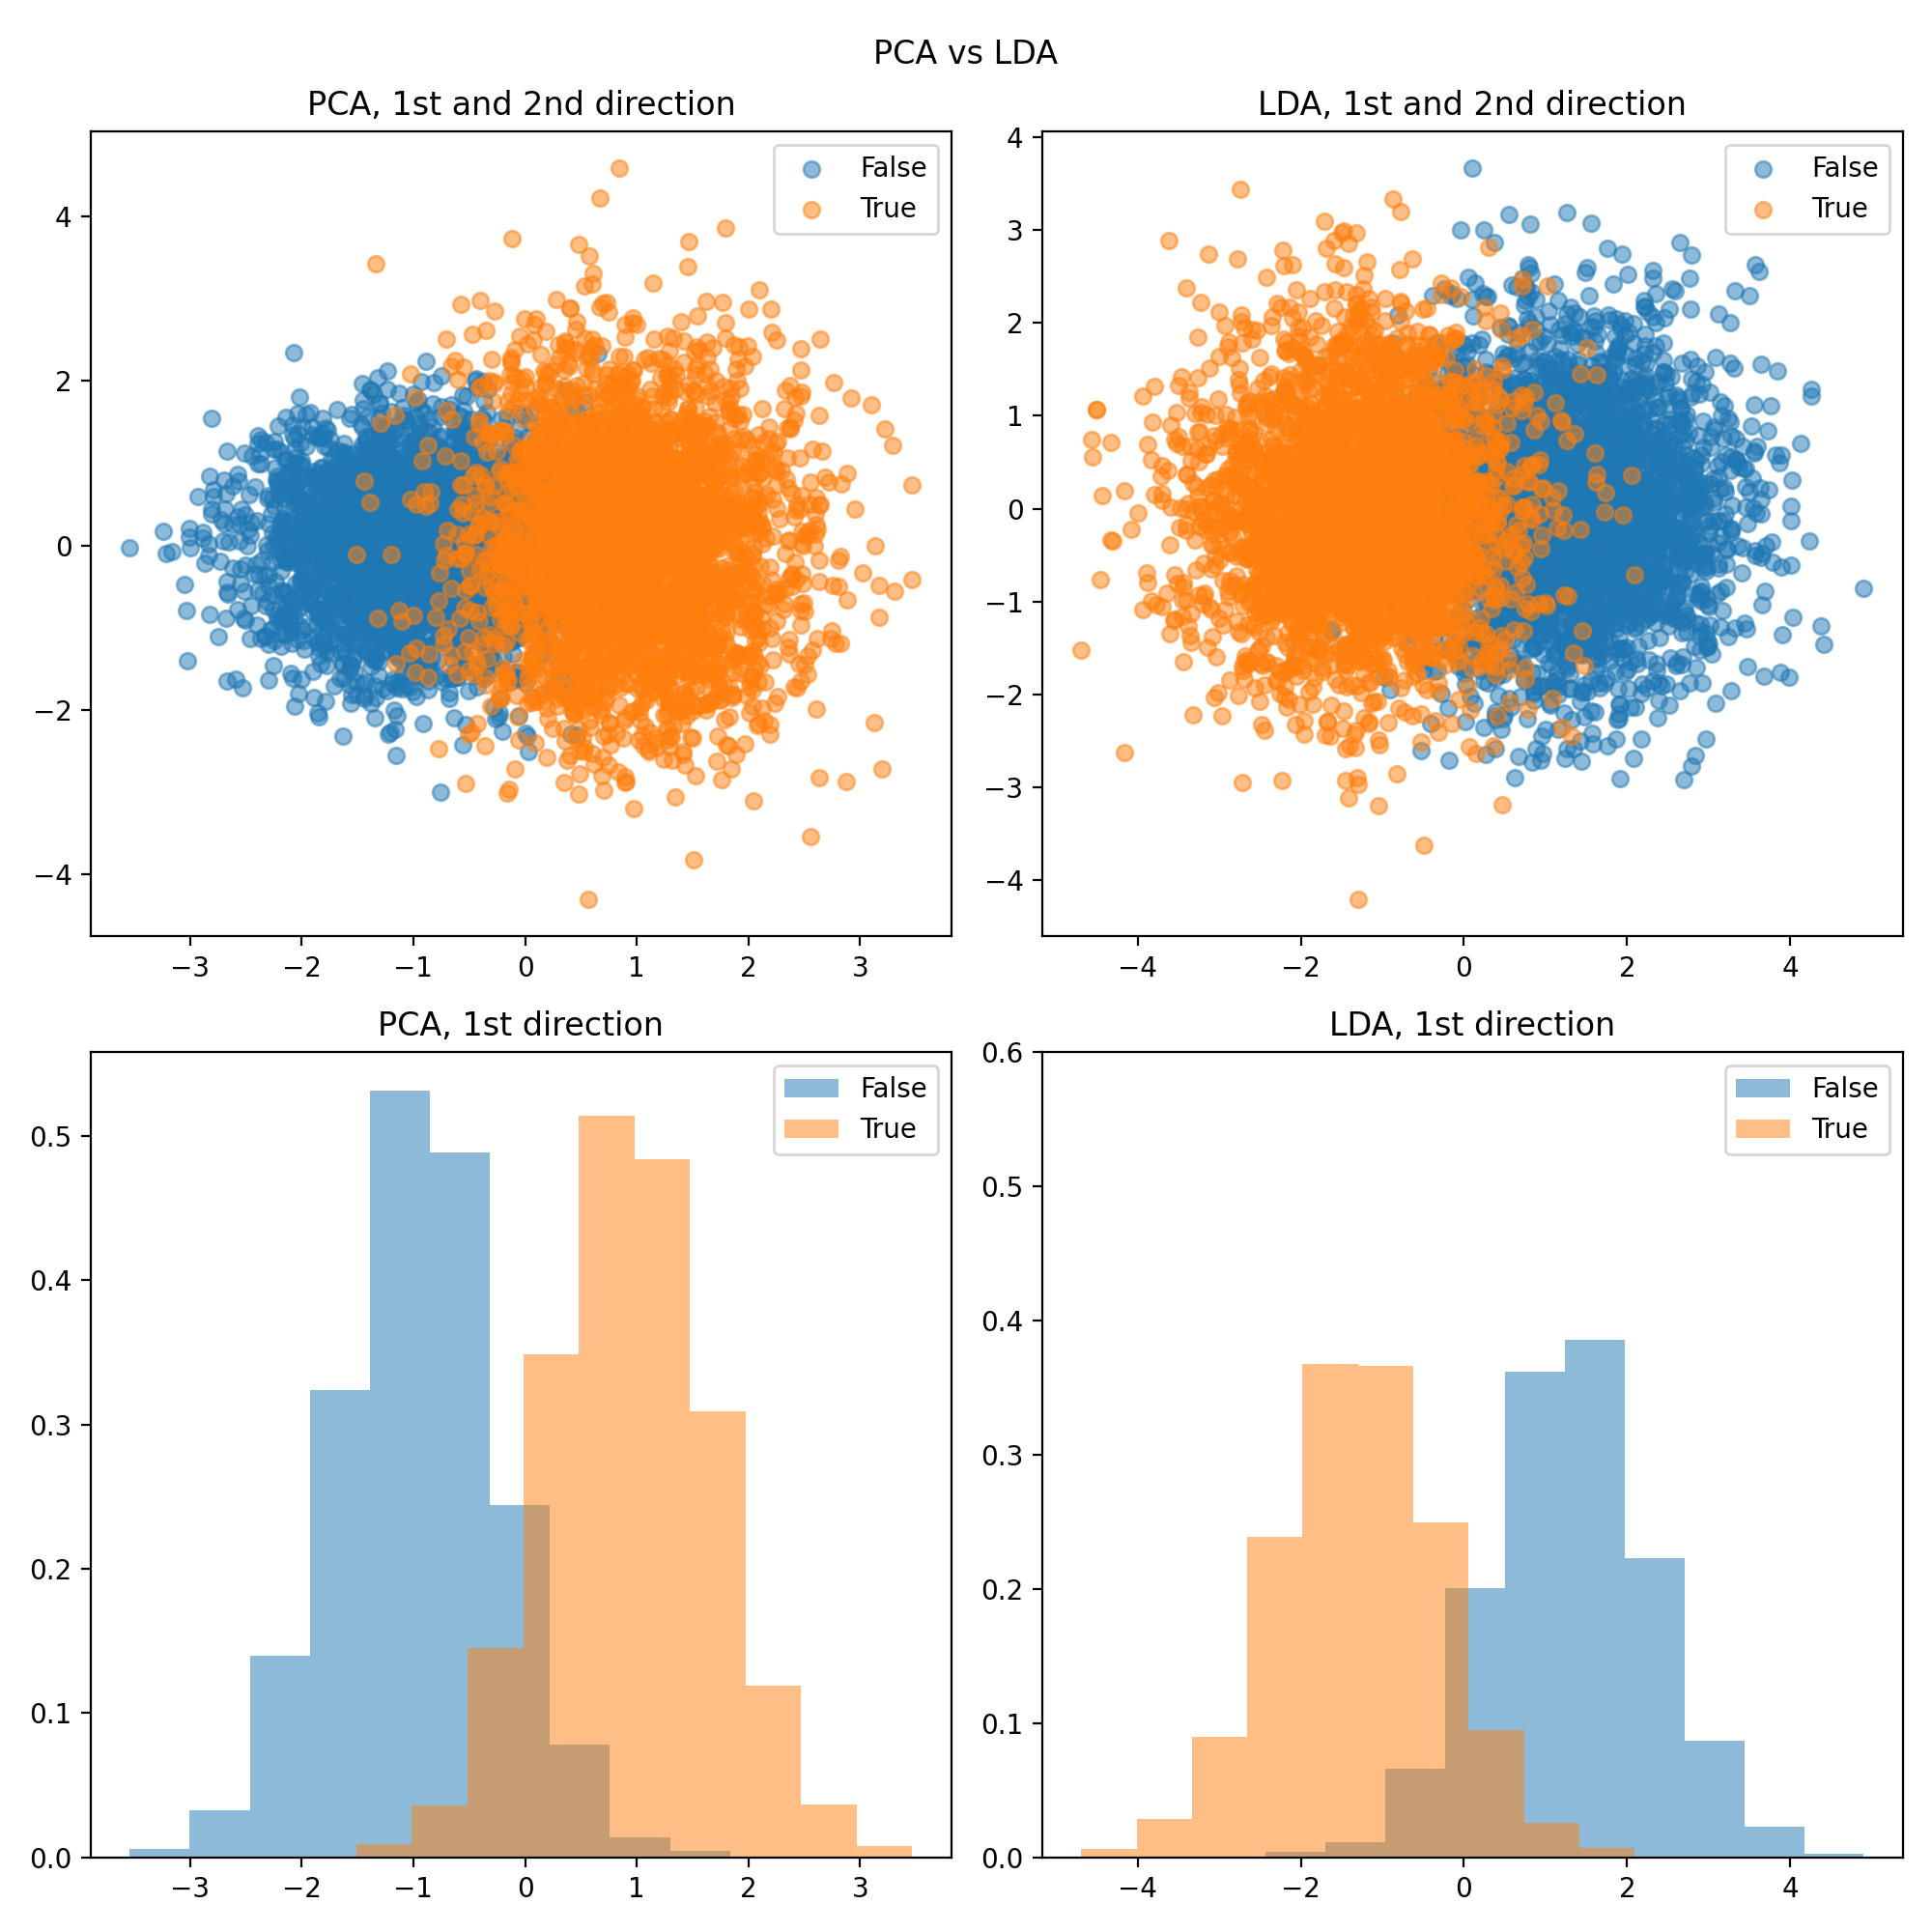
\includegraphics[width=0.5\linewidth]{Lab/03. Lab 03/Images/02. PVA_LDA}
    \caption{Comparing resulta between PCA and LDA}
    \label{fig:pcaLda}
\end{figure}

At a later stage, they were used to carry out a classification.
The available dataset was divided into two sub-portions one for training and the other for validation.
In \autoref{tab:LDAPCAForClassification} we can see the error of the classification,
errors made in the classification when varying m (only for some values) and the threshold were reported

\begin{table}
    \centering
    \begin{tabular}{c c c c}
        \toprule
        \textbf{Method}                    & \textbf{Num Samples} & \textbf{Error} & \textbf{Error Rate} (\%) \\
        \midrule
        LDA - First threshold              & 2000                 & 186            & 9.30                     \\
        LDA - Second threshold             & 2000                 & 186            & 9.30                     \\
        \midrule
        PCA (m=5) + LDA - First threshold  & 2000                 & 186            & 9.30                     \\
        PCA (m=5) + LDA - Second threshold & 2000                 & 185            & 9.25                     \\
        PCA (m=6) + LDA - First threshold  & 2000                 & 186            & 9.30                     \\
        PCA (m=6) + LDA - Second threshold & 2000                 & 184            & 9.20                     \\
        \bottomrule
    \end{tabular}
    \captionsetup{justification=justified,singlelinecheck=false,format=hang}
    \caption{Table showing the results of the LDA and PCA + LDA method for classification.}
    \label{tab:LDAPCAForClassification}
\end{table}










%    Multivariate Gaussian Density


    \section{Multivariate Gaussian Density}
    \label{sec:multivariateGaussianDensity}
    %! Author = antonio
%! Date = 7/2/24

Multivariate Gaussian Density is an extension of the Gaussian Density to multiple dimensions.
It is used to describe the distribution of a vector of random variables in a \(multi-dimensional\) space,
and it could be defined as:
\begin{equation}
    N(x\mid\mu, \Sigma) = \frac{1}{(2\pi)^{\frac{M}{2}} \left|\Sigma \right|^{\frac{1}{2}}}\exp^{-\frac{1}{2}(x-\mu)^T\Sigma^{-1}(x-\mu)}
    \label{eq:gaussianDensity}
\end{equation}

where \(M\) is the size of the feature vector \(x\), and \(\left|\Sigma \right|\) is the determinant of \(\Sigma\).
Since the computation of the exponential could cause problems, the logarithm is applied, so from \autoref{eq:gaussianDensity}
we get \autoref{eq:logGaussianDensity}:

\begin{equation}
    \log N(x\mid\mu, \Sigma) = -\frac{M}{2}\log(2\pi) - \frac{1}{2}\log\left|\Sigma \right| - \frac{1}{2}(x-\mu)^T\Sigma^{-1}(x-\mu)
    \label{eq:logGaussianDensity}
\end{equation}

\begin{figure}[h]
    \centering
    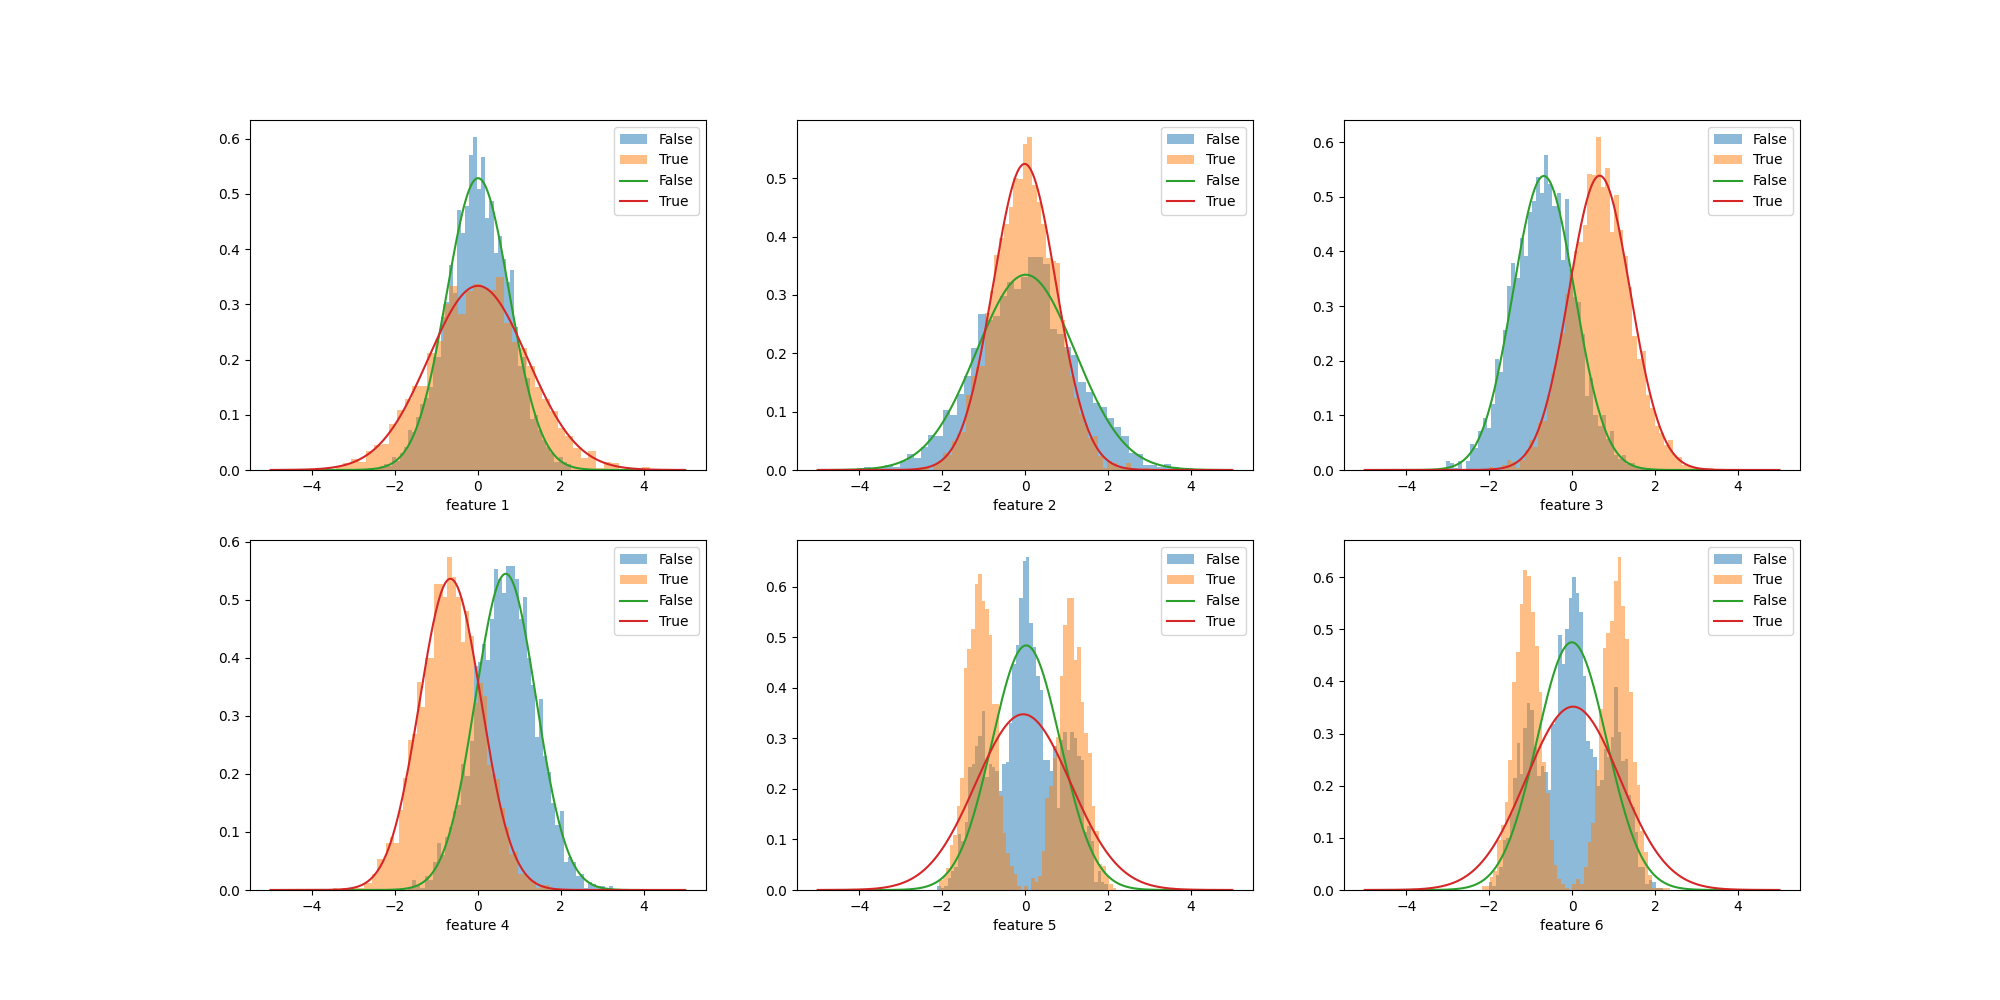
\includegraphics[width=1\linewidth]{Lab/04. Lab 04/Images/01. GaussianDensity}
    \caption{Gaussian Density}
    \label{fig:gaussianDensity}
\end{figure}

Thus, applying Gaussian probability density to the 6 features in our dataset, the following results in \autoref{fig:gaussianDensity},
are obteinded.\\
It can observe that \textbf{features 1 - 2 - 3 - 4} fit the Gaussian distribution,  the histogram of the data is well
approximated by the Gaussian curve.
For \textbf{features 5 - 6} this does not happen and therefore could not be a good model.

%    Classification Models


    \section{Classification Models Analysis}
    \label{sec:classificationModels}
    %! Author = antonio
%! Date = 7/2/24

To perform the classification, the dataset must first be divided into two sub-portions, the training and validation sub-portions.

\subsection{Gaussian models}
\label{subsec:gaussianModels}
Since, it is dealing with a binary classification task, it will assign a probabilistic score to each sample in terms
of the class-posterior log-ratio:
\begin{equation}
    \log r(x_t) = \log \frac{P(C=h_1\mid x_t)}{P(C=h_0\mid x_t)}
    \label{eq:llr}
\end{equation}

Analysing \autoref{eq:llr} in more detail, it becomes:
\begin{equation}
    \log r(x_t) = \log \frac{f_{X\mid C}(x_t \mid h_1)}{f_{X\mid C}(x_t \mid h_0)} + \log \frac{P(C=h_1)}{P(C=h_0)}
    \label{eq:llrExpanded}
\end{equation}

The first addend of the equation is called the \textit{llr} or \textit{log-likelihood ratio} and an optimal decision is
given by \autoref{eq:llrDecision}.

\begin{equation}
    \log r(x_t) \gtrless 0
    \label{eq:llrDecision}
\end{equation}

Considering \(P(C=h_1) = \pi \) and \(P(C=h_0) = 1 - \pi\), from \autoref{eq:llrExpanded} and \autoref{eq:llrDecision},
it is possible to write that the class assignment is based on \autoref{eq:llrExpanded} and \autoref{eq:llrDecision},
to obtain \autoref{eq:assignmentClasses}.

\begin{equation}
    llr(x_t)=\log \frac{f_{X\mid C}(x_t \mid h_1)}{f_{X\mid C}(x_t \mid h_0)} \gtrless -\log \frac{\pi}{1 - \pi}
    \label{eq:assignmentClasses}
\end{equation}

%   Multivariate Gaussian Classifier

\subsubsection{Multivariate Gaussian Classifier}
\label{subsubsec:multivariateGaussianClassifier}
The first classifier is given by the empirical mean and covariance of each class,
\begin{equation}
    \mu_c^* = \frac{1}{N_c} \sum_{i\mid c_i=c} x_i\text{ ,}\quad
    \Sigma_c^* = \frac{1}{N_c} \sum_{i\mid c_i=c} (x_i - \mu_c^*)(x_i - \mu_c^*)^T
    \label{eq:meanAndVarianceMVG}
\end{equation}

%   Naive Bayes Gaussian Classifier

\subsubsection{Naive Bayes Gaussian Classifier}
\label{subsubsec:naiveBayesGaussianClassifier}
This model makes an important assumption that simplifies the number of parameters to be estimated,
it assumes that the features are indepenent given their class.
This causes the covariance matrix to be a diagonal matrix, consequently, matching MVG with the diagonal covariance matrix.
However, the assumption of independence may be too restrictive and lead to inferior performance if the features are indeed correlated.

\begin{equation}
    \mu_{c,[j]}^* = \frac{1}{N_c} \sum_{i\mid c_i = c} x_{i,[j]}\text{ ,}\quad
    \sigma_{c,[j]}^2 = \frac{1}{N_c} \sum_{i\mid c_i = c} (x_{i,[j]} - \mu_{c,[j]}^*)^2
    \label{eq:meanAndVarianceNBG}
\end{equation}

%   Tied Covariance Gaussian Classifier

\subsubsection{Tied Covariance Gaussian Classifier}
\label{subsubsec:tiedCovarianceGaussianClassifier}
The assumption of the latter model consists of its own average for each class, but an equal covariance matrix for all classes.

\begin{equation}
    \mu_c^* = \frac{1}{N_c} \sum_{i\mid c_i=c} x_i\text{ ,}\quad
    \Sigma^* = \frac{1}{N} \sum_{c} \sum_{i\mid c_i = c} (x_{i} - \mu_c)(x_{i} - \mu_c)^T
    \label{eq:tiedCovariance}
\end{equation}

\subsubsection{Gaussian Models Comparison}
\label{subsubsec:gaussianModelsComparison}

    % Lab 06 NO PROJECT PART

%   Performance of Classifier
    %! Author = anton
%! Date = 28/08/2024

Starting with the previous performance, it may be interesting to analyse how performance changes as three main
parameters vary:
\begin{itemize}
    \item \(\tilde{\pi}\): represents prior probability of the positive class
    \item \(C_{fn}\): misclassification cost of a sample predicted as negative but it is positive
    \item \(C_{fp}\): misclassification cost of a sample predicted as positive but it is negative
\end{itemize}

\begin{table}[h]
    \centering
    \begin{tabular}{>{\centering\arraybackslash}p{2.9cm} >{\centering\arraybackslash}p{2.9cm} >{\centering\arraybackslash}p{2.9cm} >{\centering\arraybackslash}p{2.9cm}}
        \toprule
        & \textbf{MVG} & \textbf{Naive Bayes} & \textbf{Tied Covariance} \\
        \midrule
        \multicolumn{4}{c}{\textbf{Application \((\tilde{\pi},C_{fn}, C_{fp}) = (0.5, 1, 1)\)}} \\
        \midrule
        \textbf{actDCF} & 0.1399       & 0.1439               & 0.1860                   \\
        \textbf{minDCF} & 0.1302       & 0.1311               & 0.1812                   \\
        \midrule
        \multicolumn{4}{c}{\textbf{Application \((\tilde{\pi},C_{fn}, C_{fp}) = (0.9, 1, 1)\)}} \\
        \midrule
        \textbf{actDCF} & 0.4001       & 0.3893               & 0.4626                   \\
        \textbf{minDCF} & 0.3423       & 0.3509               & 0.4421                   \\
        \midrule
        \multicolumn{4}{c}{\textbf{Application \((\tilde{\pi},C_{fn}, C_{fp}) = (0.1, 1, 1)\)}} \\
        \midrule
        \textbf{actDCF} & 0.3051       & 0.3022               & 0.4061                   \\
        \textbf{minDCF} & 0.2629       & 0.2569               & 0.3628                   \\
        \midrule
        \multicolumn{4}{c}{\textbf{Application \((\tilde{\pi},C_{fn}, C_{fp}) = (0.5, 1, 9)\)}} \\
        \midrule
        \textbf{actDCF} & 0.3051       & 0.3022               & 0.4061                   \\
        \textbf{minDCF} & 0.2629       & 0.2569               & 0.3628                   \\
        \midrule
        \multicolumn{4}{c}{\textbf{Application \((\tilde{\pi},C_{fn}, C_{fp}) = (0.5, 9, 1)\)}} \\
        \midrule
        \textbf{actDCF} & 0.4001       & 0.3893               & 0.4626                   \\
        \textbf{minDCF} & 0.3423       & 0.3509               & 0.4421                   \\
        \bottomrule
    \end{tabular}
    \captionsetup{justification=justified,singlelinecheck=false,format=hang}
    \caption{Table showing minDCF and actDCF for different models and applications.}
    \label{tab:resultPerformanceClassifierWithoutPCA}
\end{table}

Analysing the results of the \autoref{tab:resultPerformanceClassifierWithoutPCA}, it is possible to observe:

\begin{table}[h]
    \centering
    \begin{tabular}{>{\centering\arraybackslash}p{2.9cm} >{\centering\arraybackslash}p{2.9cm} >{\centering\arraybackslash}p{2.9cm} >{\centering\arraybackslash}p{2.9cm}}
        \toprule
        & \textbf{MVG} & \textbf{Naive Bayes} & \textbf{Tied Covariance} \\
        \toprule
        \toprule
        \multicolumn{4}{c}{\textbf{Application \((\tilde{\pi},C_{fn}, C_{fp}) = (0.5, 1, 1)\)}} \\
        \midrule
        \multicolumn{4}{c}{\textbf{no PCA}} \\
        \midrule
        \textbf{actDCF} & 0.1399       & 0.1439               & 0.1860                   \\
        \textbf{minDCF} & 0.1302       & 0.1311               & 0.1812                   \\
        \midrule
        \multicolumn{4}{c}{\textbf{PCA}} \\
        \multicolumn{4}{c}{\textbf{\(m = 5\)}} \\
        \midrule
        \textbf{actDCF} & 0.1419       & 0.1749               & 0.1860                   \\
        \textbf{minDCF} & 0.1331       & 0.1737               & 0.1812                   \\
        \midrule
        \multicolumn{4}{c}{\textbf{\(m = 6\)}} \\
        \midrule
        \textbf{actDCF} & 0.1399       & 0.1780               & 0.1860                   \\
        \textbf{minDCF} & 0.1302       & 0.1727               & 0.1812                   \\
        \toprule
        \toprule
        \multicolumn{4}{c}{\textbf{Application \((\tilde{\pi},C_{fn}, C_{fp}) = (0.9, 1, 1)\)}} \\
        \midrule
        \multicolumn{4}{c}{\textbf{no PCA}} \\
        \midrule
        \textbf{actDCF} & 0.4001       & 0.3893               & 0.4626                   \\
        \textbf{minDCF} & 0.3423       & 0.3509               & 0.4421                   \\
        \midrule
        \multicolumn{4}{c}{\textbf{PCA}} \\
        \multicolumn{4}{c}{\textbf{\(m = 5\)}} \\
        \midrule
        \textbf{actDCF} & 0.3980       & 0.4660               & 0.4626                   \\
        \textbf{minDCF} & 0.3512       & 0.4340               & 0.4451                   \\
        \midrule
        \multicolumn{4}{c}{\textbf{\(m = 6\)}} \\
        \midrule
        \textbf{actDCF} & 0.4001       & 0.4512               & 0.4626                   \\
        \textbf{minDCF} & 0.3423       & 0.4359               & 0.4421                   \\
        \toprule
        \toprule
        \multicolumn{4}{c}{\textbf{Application \((\tilde{\pi},C_{fn}, C_{fp}) = (0.1, 1, 1)\)}} \\
        \midrule
        \multicolumn{4}{c}{\textbf{no PCA}} \\
        \midrule
        \textbf{actDCF} & 0.3051       & 0.3022               & 0.4061                   \\
        \textbf{minDCF} & 0.2629       & 0.2569               & 0.3628                   \\
        \midrule
        \multicolumn{4}{c}{\textbf{PCA}} \\
        \multicolumn{4}{c}{\textbf{\(m = 5\)}} \\
        \midrule
        \textbf{actDCF} & 0.3042       & 0.3930               & 0.4051                   \\
        \textbf{minDCF} & 0.2738       & 0.3545               & 0.3648                   \\
        \midrule
        \multicolumn{4}{c}{\textbf{\(m = 6\)}} \\
        \midrule
        \textbf{actDCF} & 0.3051       & 0.3920               & 0.4061                   \\
        \textbf{minDCF} & 0.2629       & 0.3535               & 0.3628                   \\
        \bottomrule
    \end{tabular}
    \captionsetup{justification=justified,singlelinecheck=false,format=hang}
    \caption{Show minDCF and actDCF for different models and applications before and after applying PCA.}
    \label{tab:resultPerformanceClassifierWithPCA}
\end{table}

\begin{figure}[h!]
    \centering
    \begin{subfigure}[b]{0.4\linewidth}
        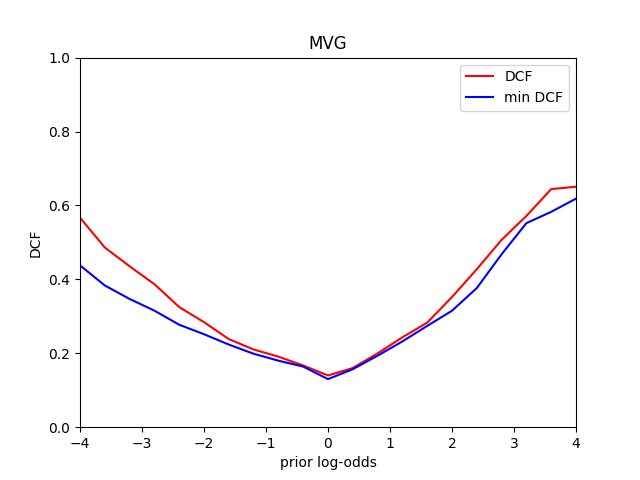
\includegraphics[width=\linewidth]{Lab/07. Lab 07/Images/01. MVG}
        \caption{Without mean}
        \label{fig:dcfMVG}
    \end{subfigure}
    \begin{subfigure}[b]{0.4\linewidth}
        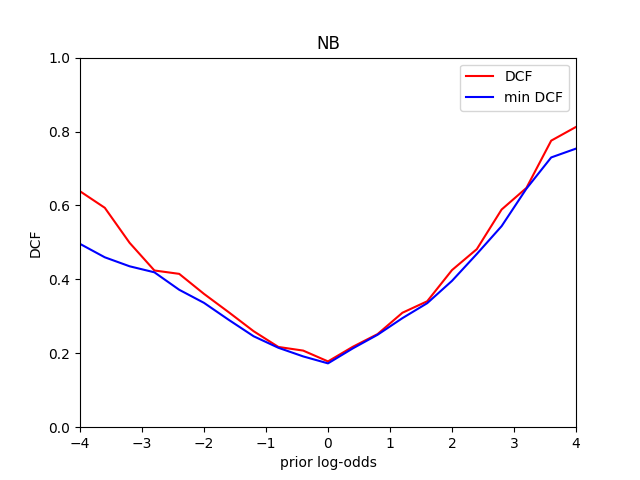
\includegraphics[width=\linewidth]{Lab/07. Lab 07/Images/02. Naive Bayes}
        \caption{With mean}
        \label{fig:dcfNB}
    \end{subfigure}
    \begin{subfigure}[b]{0.4\linewidth}
        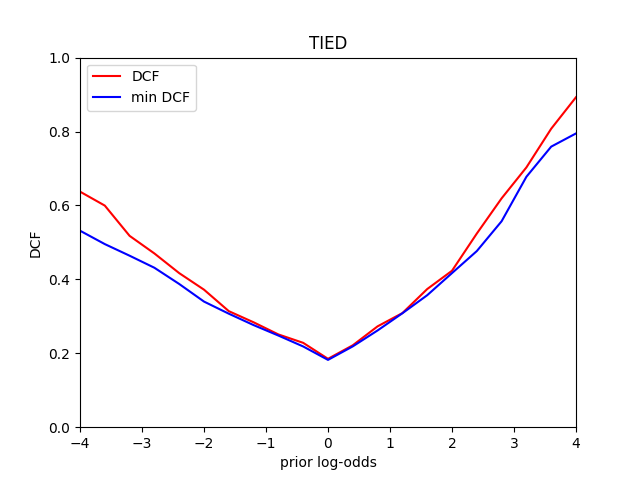
\includegraphics[width=\linewidth]{Lab/07. Lab 07/Images/03. Tied}
        \caption{With mean}
        \label{fig:dcfTC}
    \end{subfigure}
    \caption{}
    \label{fig:dcfMVGNBTC}
\end{figure}


\end{document}
